\documentclass[12pt]{article}
\usepackage{amsmath}
\usepackage{amssymb}
\usepackage{tikz}
\usepackage{float}
\usepackage{enumitem}
\usepackage{url}
\usepackage{microtype}
\usepackage{graphicx}
\usepackage[style=ieee,backend=bibtex]{biblatex}
\usetikzlibrary{arrows}
\usetikzlibrary{arrows.meta}
\bibliography{gopher-brain}
\begin{document}

\title{gopher-brain}
\author{Matthew T. R.}
\date{\today{}}
\maketitle{}

\newpage

\tableofcontents{}

\newpage

\section*{Abstract} \label{abstract}

Yet to be written.

\section{Introduction} \label{intro}

From a computational standpoint, each neuron in the brain can be described as an individual agent \cite{agentbased}.  Thus, we can potentially model a neural system around agent-based modeling.  Additionally, it has been established that we can use a simple form of learning \cite{agentbased} to assist in this model.  However, this only answers the question of continual learning.  From a biological standpoint, we can see that multiple organisms have a "critical phase" for learning \cite{neurodev} and have distinct rates of synaptogenesis and synaptic pruning throughout their lifetimes.  Additionally, organisms may combine various environmental factors into their decision making - "senses".  Here, we explore the interplay between multiple inputs and synaptic modification.

There are types of neural networks called recurrent neural networks, in which nodes may connect both "backwards" and "forwards"; however, in an animal brain, there is no real concept of "backwards" or "forwards".  Rather, there are a plethora of inputs and a plethora of outputs.  Based on this range of input and output methods, we know that two apparently unrelated outputs can affect the resulting input, or two inputs can affect the resulting output (e.g. legs and arms, and sight and sound, respectively), which is the primary focus of this investigation.

Throughout this paper, we refer to both "neurons" and "nodes", defined as the same thing, and "axons", "synapses", and "connections", where a connection is the composite of a neuron's single axon and that axon's outgoing synapses.  "Weights" and "strengths" of synapses mean the same thing.

\newpage

\section{Simulation} \label{simulation}

First, we developed an appropriate simulation using a custom agent-based model, which is described here.  Once that was completed, we translated that into its equivalent mathematical models, discussed in Section 3.

\subsection{Setup} \label{setup}

We begin by generating a three-dimensional grid of nodes given a set $\left\{x_0, y_0, z_0\right\}$.  Connections are generated randomly, with each node creating an axon with a center of some distance away from the node (see section 3).  This procedure creates one hemisphere.

To create the other hemisphere, we then create a grid using this set's dimensions and mirror this grid along the plane $x = x_0$ so that the combined grid's dimensions are $\{x_0 * 2, y_0, z_0\}$.  At this point, we have now created two hemispheres with duplicate axon centers; however, we have not yet created the actual synapses.

To create synapses, we repeat the process we devised in generating axon centers (again, see section 3).  However, we choose a smaller standard deviation.  We create synapses on the axons of all nodes in this way.  Due to the symmetric axon centers but asymmetric synapses, the two halves of the network are then similar, but not the same.

\subsection{Firing cycle} \label{cycle}

During each cycle, two primary events take place.  First, nodes have the potential to generate new synapses around their axon centers if both the originator node and the potential node to connect to both have fired on the previous cycle.  Once the nodes have created their new synapses (if any), each node runs a simple algorithm to determine whether it should fire.  Once it fires or not, it then analyzes each of its outgoing synapses, adjusting the weights based on the combination of firing neurons.  This process is highly similar to Hebbian learning.  However, there are multiple major differences, primarily regarding connections (described in the next section).

\subsection{Connections} \label{simconnections}

As alluded to previously, one node always has exactly one axon.  However, one axon may have many synapses, and those synapses then each connect to exactly one other node.  Nodes may not connect to themselves.  Axons also may move when generating new synapses to be in the center of the nodes they connect to.

These connection details are where this model differs from a standard Hebbian learning model.  First, when one node fires, it may influence muliple nodes at once, all with different signal strengths, and those individual synapses are modified (but still connected to those individual nodes).  Second, synapses may be destroyed if their strength is too weak, or created at random between two nodes that happened to fire together.  Third, the generation of synapses and axons is spatial, so a given node will tend to connect with nodes that are close to itself.

\subsection{Sensors and Outputs} \label{simio}

We call any external input to the network a "sensor".  To generate a sensor, we pick a center and create a probability sphere in which affected nodes may be located, much like axon centers and synapses are generated.  We expect some outside program to do the input processing, as it's not up to the network what happens with its outputs.  Output neuron clusters are generated in the same way, and for now, just have their individual values to the sum of their neurons.  However, each neuron does have a separate synapse on the axon specifically for the output(s) it's tied to, so the output neurons do affect the output value with different strengths.

\newpage

\section{Formalization and Abstraction} \label{formal}

A partial definition of our developed system has been designed within the program as a matrix of arrays

$$
\left(\begin{array}{cccc}
{[n_{000}, ..., n_{00z}]} & {[n_{100}, ..., n_{10z}]} & ... & {[n_{x00}, ..., n_{x0z}]} \\
{[n_{010}, ..., n_{01z}]} & {[n_{110}, ..., n_{11z}]} & ... & {[n_{x10}, ..., n_{x1z}]} \\
... & ... &... & ... \\
{[n_{0y0}, ..., n_{0yz}]} & {[n_{1y0}, ..., n_{1yz}]} & ... & {[n_{xy0}, ..., n_{xyz}]}
\end{array} \right)
$$

Alternatively, the network can be described as a large digraph
$$
\bordermatrix{
        & n_0 & n_1 & ... & n_n \cr
    n_0 & \o & w_{01} & ... & w_{0n} \cr
    n_1 & w_{01} & \o & ... & w_{1n} \cr
    ... & ... & ... & ... & ... \cr
    n_n & w_{0n} & w_{1n} & ... & \o } \qquad
$$

Where $n_n$ is the $n^{th}$ node and $w_{ij}$ is the weight of the connection from node $i$ to node $j$, although this description loses the position of each node while gaining synapse information.

Within our simulation, each node stores its value and its axon, and each axon in turn stores an array of nodes it's connected to.  Due to this, we could in theory generate a complete adjacency matrix; however, at the scale we work at (often tens of thousands of nodes, caused by the three dimensions), this is impractical.

\subsection{Axons and Synapses} \label{connections}

To generalize, we may create a three-dimensional "probability sphere" with a normal Gaussian distribution around the center as follows
$$\left\{\mathcal{N}(center_x, \sigma^{2}), \mathcal{N}(center_y, \sigma^{2}), \mathcal{N}(center_z, \sigma^{2})\right\}$$
We define $\sigma_{axon\_distribution} > \sigma_{synapse\_distribution}$ so that axons may reach an arbitrarily far distance, but synapses always are generated in the immediate vicinity of the axon center.  This generation allows us to create axons and synapses such that they are always close to the center that generates them, yet still have the potential to reach out.

Any time a new synapse is created, we update the axon center to reflect the addition of the synapse by setting the center to be the average of the centers of the nodes it connects to.  Generally, $c_i = \frac{1}{p}\sum c_{ki}$ where $c_i$ is the $i^{th}$ component of the center point for any given dimensionality and $c_{ki}$ is the $i^{th}$ component of the $k^{th}$ node's center.

\subsection{Neurons} \label{neurons}

We define the sum of a neuron to be
$$n_{nv} \propto \sum (n_{ie} * n_{iv} * n_{inw})$$
where $n_{nv}$ is the node value, $n_{niv}$ is the value of node i, $n_{ie}$ is the excitatory status of a node, and $n_{niw}$ is the weight, or strength, of the connection from node i to node n.
Nodes either fire as 1 or 0, and we define a node as "firing" as soon as $n_{nv} >= 1$.  On the other hand, if $n_{nv} < 1$, the node, like a neuron, doesn't fire.  Thus, $n_{iv} \in \{0, 1\}$.  Additionally, $n_{ie} \in \{-1, 1\}$ and determines whether a node is excitatory or inhibitory.

Once we determine which nodes have fired, we can then modify connections based on the firing status of various nodes.  Our devised formula for this is
$$
\Delta w_{ij} =
\begin{cases}
g, n_i = n_j = 1\\
-l, n_i \neq n_j\\
-d, n_i = n_j = 0
\end{cases}
$$

Where $g$ is the growth factor or function, $l$ is the loss factor or function, and $d$ is the decay factor or function.  For our simulation, we chose $d < l$ so that connections decay more slowly if neither neuron is active.  In some cases, $l$ may be defined as 0; however, this would lead to never pruning unused neurons.

Additionally, we choose to have endpoints such that $w_{ij} \in [c_0, c_1]$ so that no single connection becomes overly strong or weak.  Because $c_0$ is defined as the minimum strength, we remove any connections $w_{ij} < c_0$.

\subsection{Sensors and Outputs} \label{formalio}

Much like neuron sums, we can define the sum of a given output $o$ to be

$$
o_s = \sum (n_{ie} * n_{iv} * n_{iw})
$$

where $o_s$ is the final output value,  $n_{iv}$ is the value of the $i^{th}$ neuron, $n_{ie}$ is the excitatory status of the neron, and $n_{iw}$ is the strength of the neuron's connection to the output.

\begin{figure}[H]
    \centering
    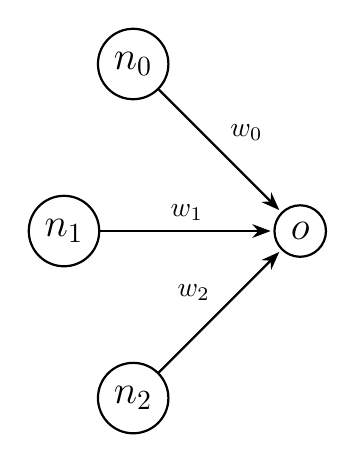
\begin{tikzpicture}[->,>=stealth',shorten >=1pt,auto,node distance=3cm,
                        thick,main node/.style={circle,draw,font=\sffamily\Large\bfseries}]

        \node[main node] (output) {$o$};
        \node[main node] (n0) [above left of=output] {$n_0$};
        \node[main node] (n1) [left of=output] {$n_1$};
        \node[main node] (n2) [below left of=output] {$n_2$};
        \begin{scope}[>={Stealth[black]}]
            \path [->] (n0) edge node {$w_{0}$} (output);
            \path [->] (n1) edge node {$w_{1}$} (output);
            \path [->] (n2) edge node {$w_{2}$} (output);
        \end{scope}
    \end{tikzpicture}
    \caption{Output} \label{fig:Output}
\end{figure}

In our model, outputs are generated the same way synapse clusters are.  We pick a center and pick $n$ nodes around the center based on a three-dimensional Gaussian distribution with standard deviation $\sigma_o$.

Sensors allow us to define any function that affect the neurons that are part of the given sensors, defining $n_{iv} = s(n_i)$ where $n_i$ is the $i$th node and $n_{iv}$ is the $i$th node's value.

\begin{figure}[H]
    \centering
    \begin{tikzpicture}[->,>=stealth',shorten >=1pt,auto,node distance=3cm,
                        thick,main node/.style={circle,draw,font=\sffamily\Large\bfseries}]

        \node[main node] (sensor) {$s$};
        \node[main node] (n0) [above right of=output] {$n_0$};
        \node[main node] (n1) [right of=output] {$n_1$};
        \node[main node] (n2) [below right of=output] {$n_2$};
        \begin{scope}[>={Stealth[black]}]
            \path [->] (sensor) edge node {$s(n_0)$} (n0);
            \path [->] (sensor) edge node {$s(n_1)$} (n1);
            \path [->] (sensor) edge node {$s(n_2)$} (n2);
        \end{scope}
    \end{tikzpicture}
    \caption{Example Sensor} \label{fig:Sensor}
\end{figure}

\begin{figure}[H]
    \centering
    \begin{tikzpicture}[->,>=stealth',shorten >=1pt,auto,node distance=3cm,
                        thick,main node/.style={circle,draw,font=\sffamily\Large\bfseries}]

        \node[main node, fill=black, text=white] (environment) [below left of=output] {$e$};
        \node[main node] (outputs) [left of=environment] {$o$};
        \node[main node] (inputs) [right of=environment] {$i$};
        \node[main node] (network) [below of=environment] {$n$};
        \begin{scope}[>={Stealth[black]}]
            \path [->] (outputs) edge node {} (environment);
            \path [->] (outputs) edge[bend right=20] node {} (environment);
            \path [->] (outputs) edge[bend left=20] node {} (environment);
            \path [->] (outputs) edge[bend left=40] node {} (environment);
            \path [->] (outputs) edge[bend right=40] node {} (environment);

            \path [->] (environment) edge node {} (inputs);
            \path [->] (environment) edge[bend right=20] node {} (inputs);
            \path [->] (environment) edge[bend left=20] node {} (inputs);
            \path [->] (environment) edge[bend left=40] node {} (inputs);
            \path [->] (environment) edge[bend right=40] node {} (inputs);

            \path [->] (inputs) edge[bend left=20] node {} (network);
            \path [->] (network) edge[bend left=20] node {} (outputs);
        \end{scope}
    \end{tikzpicture}
    \caption{Environment} \label{fig:Environment}
\end{figure}

Overall, we may consider the relationship between outputs $o$, inputs $i$, the environment $e$, and the network $n$.  If we describe them as functions, the inputs $i = e(n)$ so that the environment acts to transform the outputs into the inputs.  Then, we may describe the outputs $o = n(i)$ so that the outputs are a function of the inputs.  This then describes the environment as a sort of "black box" function that transforms, in some way unknown to us, outputs into inputs, and the network as a known function that transforms inputs into outputs.

\newpage

\section{Results} \label{results}

As many of our networks had at least 8000 nodes, and many runs generated at least 900 frames, it is impractical to share all node values and output values throughout every frame from every experimental run.  However, in sections \ref{outputvals} and \ref{graphs}, we provide graphs of output values over time.  Additionally, the source of our simulation is available to inspect and build at \url{https://github.com/firedrake969/gopher-brain} (with a web interface available at \url{https://github.com/firedrake969/brain-socket}).  Please note that all graphs in this section are displayed in a larger format in section \ref{graphs}.

\section{Discussion} \label{discussion}

\subsection{Symmetry} \label{symmetry}

We acknowledge that hemispheres are not symmetric \cite{hemisphereasymmetry}; however, newer research has discovered that the asymmetry in organic brains may be due to different growth rates \cite{hemispheredev} and hypothesized that more bilateral pathways may be advantageous \cite{recallasymmetry}.  Due to this newer research, we believe that our model is reasonably accurate with regards to symmetry.  Specifically, only inputs, outputs, and axon centers are symmetric, and axon centers change over time as new synapses are formed or old synapses are pruned, which eventually causes the hemispheres to lose their starting symmetry.

\subsection{Difference from RNNs} \label{rnndiff}

As alluded to in our introduction, we believe this network to be unique from Recurrent Neural Networks (RNNs).  In organic brains, outputs (primarily muscle motion) are essentially "processed" by the outside world, and fed back into the brain in the form of senses.  We can describe these multiple senses as multiple inputs in our model, with the key difference from RNNs being the variety of combinations of both inputs and outputs.  Then, we can define inputs, not necessarily distinct, arbitrarily, without being bounded by a certain input layer or a certain output layer.

Previous research has explored multidimensional RNNs \cite{dimensionalrnn} (as opposed to traditional, one-dimensional RNNs).  However, the problem at hand was that one-dimensional RNNs require one-dimensional inputs, while multidimensional RNNs may take multidimensional inputs.  But, it is known that humans receive two-dimensional images on their retinas and, from that image (generally), are able to produce three-dimensional images, signifying a automatic dimensional transformation.

\subsection{Memory and Signal Looping} \label{looping}

\begin{figure}[H]
    \centering
    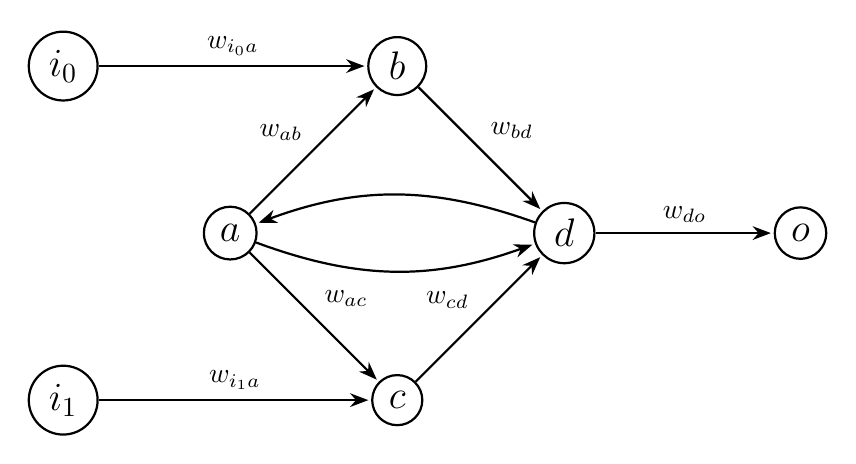
\begin{tikzpicture}[->,>=stealth',shorten >=1pt,auto,node distance=3cm,
                        thick,main node/.style={circle,draw,font=\sffamily\Large\bfseries}]

        \node[main node] (top) {$b$};
        \node[main node] (left) [below left of=top] {$a$};
        \node[main node] (bottom) [below right of=left] {$c$};
        \node[main node] (right) [below right of=top] {$d$};

        \node[main node] (inputzero) [above left of=left] {$i_0$};
        \node[main node] (inputtwo) [below left of=left] {$i_1$};
        \node[main node] (output) [right of=right] {$o$};

        \begin{scope}[>={Stealth[black]}]
            \path [->] (left) edge node {$w_{ab}$} (top);
            \path [->] (left) edge node {$w_{ac}$} (bottom);
            \path [->] (top) edge node {$w_{bd}$} (right);
            \path [->] (bottom) edge node {$w_{cd}$} (right);
            \path [->] (inputzero) edge node {$w_{i_0a}$} (top);
            \path [->] (inputtwo) edge node {$w_{i_1a}$} (bottom);
            \path [->] (right) edge node {$w_{do}$} (output);

            \path [->] (right) edge[bend right=20] node {} (left);
            \path [->] (left) edge[bend right=20] node {} (right);
        \end{scope}
    \end{tikzpicture}
    \caption{Initial} \label{fig:Initial}
\end{figure}

In Figure 1, in which $w_{ij}$ denotes the strength of the connection between nodes $i$ and $j$, we illustrate a simple system that exemplifies an instance of signal looping.  Nodes $a$ and $d$ are able to signal to each other in such a way that if one of the pair gets a signal, the other may be triggered, causing the initial node to signal again and resulting in a loop that continuously strengthens $w_{ad}$ and $w_{da}$ or, more generally, the weights between the initial and the secondary node. ($w_{ad}$ and $w_{da}$ not pictured due to space constraints)

For instance, we can imagine a scenario in which nodes $i_0$ and $i_1$ are firing, causing nodes $b$, $c$, and by extension, $a$, $d$, and $o$ to fire.  If we consider $o$ an output node, we can view this output from the combination of nodes $i_0$ and $i_1$.  Once those two stimuli cease to fire, however, $a$ can continue firing in a loop with $d$.  In this case, $i_0$ and $i_1$ may not be enough individually to cause $d$ to fire back to $a$, but in combination, their effect pushes $d$ over the threshold.

\begin{figure}[H]
    \centering
    \begin{tikzpicture}[->,>=stealth',shorten >=1pt,auto,node distance=3cm,
                        thick,main node/.style={circle,draw,font=\sffamily\Large\bfseries}]

        \node[main node] (left) {$a$};
        \node[main node] (right) [left of=top] {$d$};

        \begin{scope}[>={Stealth[black]}]
            \path [->] (right) edge[bend right=20] node {} (left);
            \path [->] (left) edge[bend right=20] node {} (right);
        \end{scope}
    \end{tikzpicture}
    \caption{Stuck in a loop} \label{fig:Stuck in a loop}
\end{figure}

\begin{figure}[H]
    \centering
    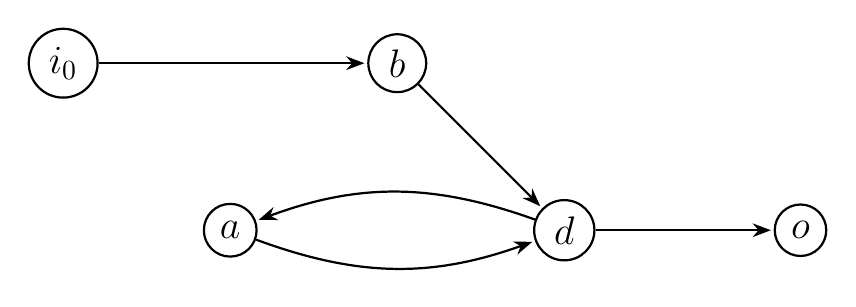
\begin{tikzpicture}[->,>=stealth',shorten >=1pt,auto,node distance=3cm,
                        thick,main node/.style={circle,draw,font=\sffamily\Large\bfseries}]

        \node[main node] (top) {$b$};
        \node[main node] (left) [below left of=top] {$a$};
        \node[main node] (right) [below right of=top] {$d$};

        \node[main node] (inputzero) [above left of=left] {$i_0$};
        \node[main node] (output) [right of=right] {$o$};

        \begin{scope}[>={Stealth[black]}]
            \path [->] (inputzero) edge node {} (top);
            \path [->] (top) edge node {} (right);
            \path [->] (right) edge node {} (output);
            \path [->] (right) edge[bend right=20] node {} (left);
            \path [->] (left) edge[bend right=20] node {} (right);
        \end{scope}
    \end{tikzpicture}
    \caption{Input} \label{fig:Input}
\end{figure}

Then, with this signal looping between neurons, we can cause a signal from either $i_0$ or $i_1$ to generate another output to $o$ (see Figure 3).  In this way, we have created a system which initially requires multiple inputs, yet after reaching a certain number of inputs, requires fewer inputs.  This can be generalized to include subsystems of nodes in place of the individual nodes illustrated, due to the previously described neuron firing definition. (describe more)

Due to this generalization, we can argue that the network has a sort of "memory" - after receiving a set of inputs, the system may generate the same, or similar, output after receiving one (or part) of the same set of inputs; that is, once the input set $m$ is received and outputs $o$, $m_0$ can be received where $m_0 \subseteq m$ and the subsequent output is $o_0 \simeq o$.  As described previously, this is distinct from RNNs as it can combine distinct inputs.  This concept has previously been explored in a biological setting \cite{synapsememory}.

\subsection{Priming} \label{priming}

We provide a function, callable at any time, that randomizes the values of all nodes, with a 50\% chance of any given node being in an active state.  This randomization, or priming, does not take into account hemisphere symmetry.  However, it is still useful in that we may randomize initially to determine both the interplay of sensor inputs on a chaotic network and the lack of any inputs on a chaotic network.

\begin{figure}[H]
    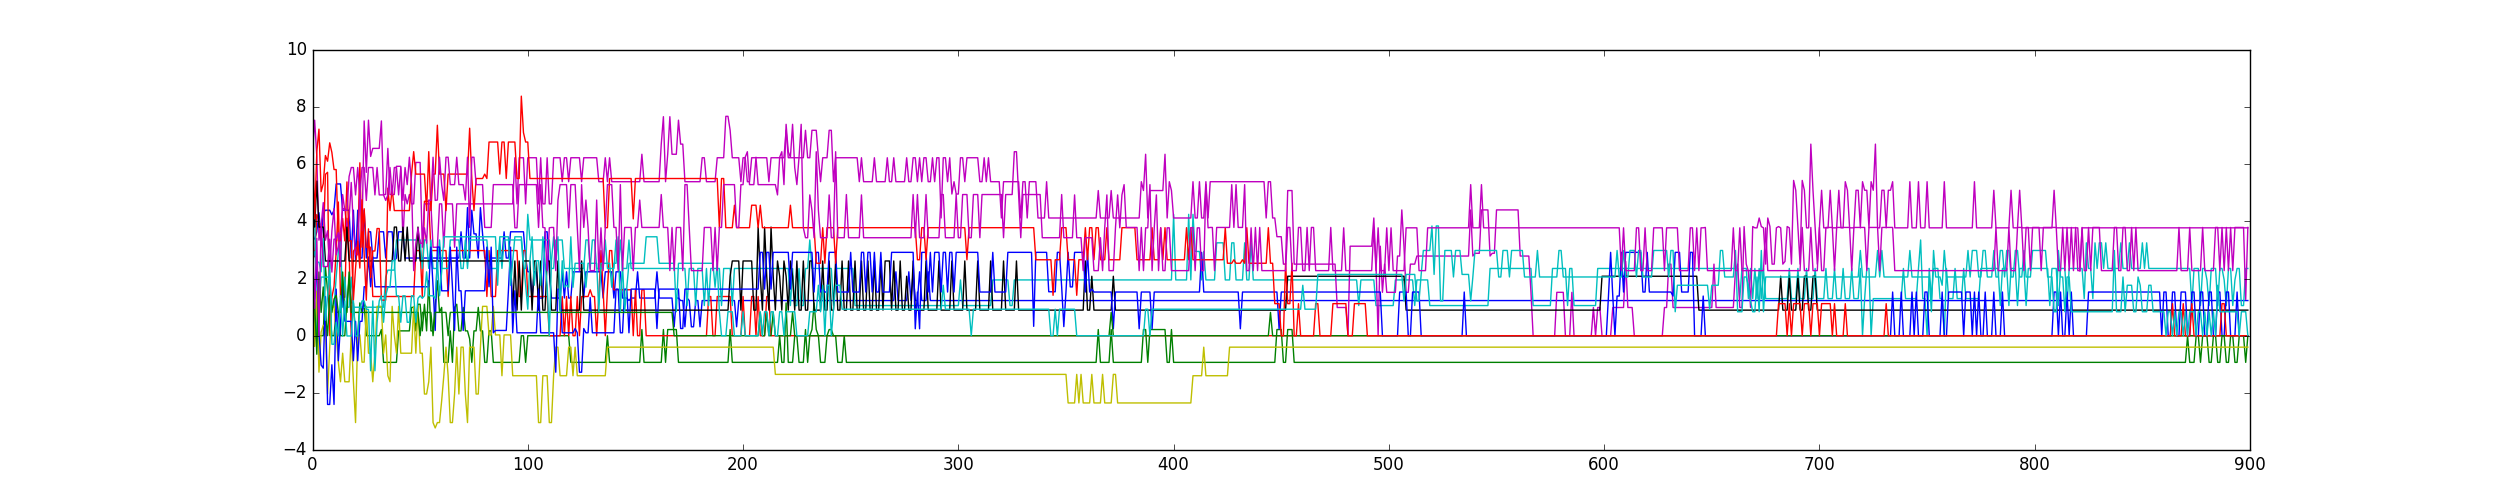
\includegraphics[width=\linewidth]{../visualizations/8knodes_stable_line.png}
    \caption{Randomized (no inputs)}
    % \label{fig:unprimed_sensoroutput_graph}
\end{figure}

This figure illustrates the values of various outputs without any sensory input, over 900 cycles (note that there are two pink lines).  Visually, we can see that the values of the outputs have high fluctuation within the first 100 frames, and then settle into repetitions  between two values.  Although originally chaotic, a stable point is eventually reached with a lack of any input.

The drawback of randomizing the entire network is that it's random - there's no symmetry between hemispheres, much less any order.  We chose to randomize the entire network because we can allow the network to cycle until we feel that the output values have begun looping within a set range.  However, it's possible that we may not need to randomize this in the future if we decide to create numerous sensors, feeding to different areas in the network, allowing for much more input at any given time.

\subsection{Output Values} \label{outputvals}

\begin{figure}[H]
    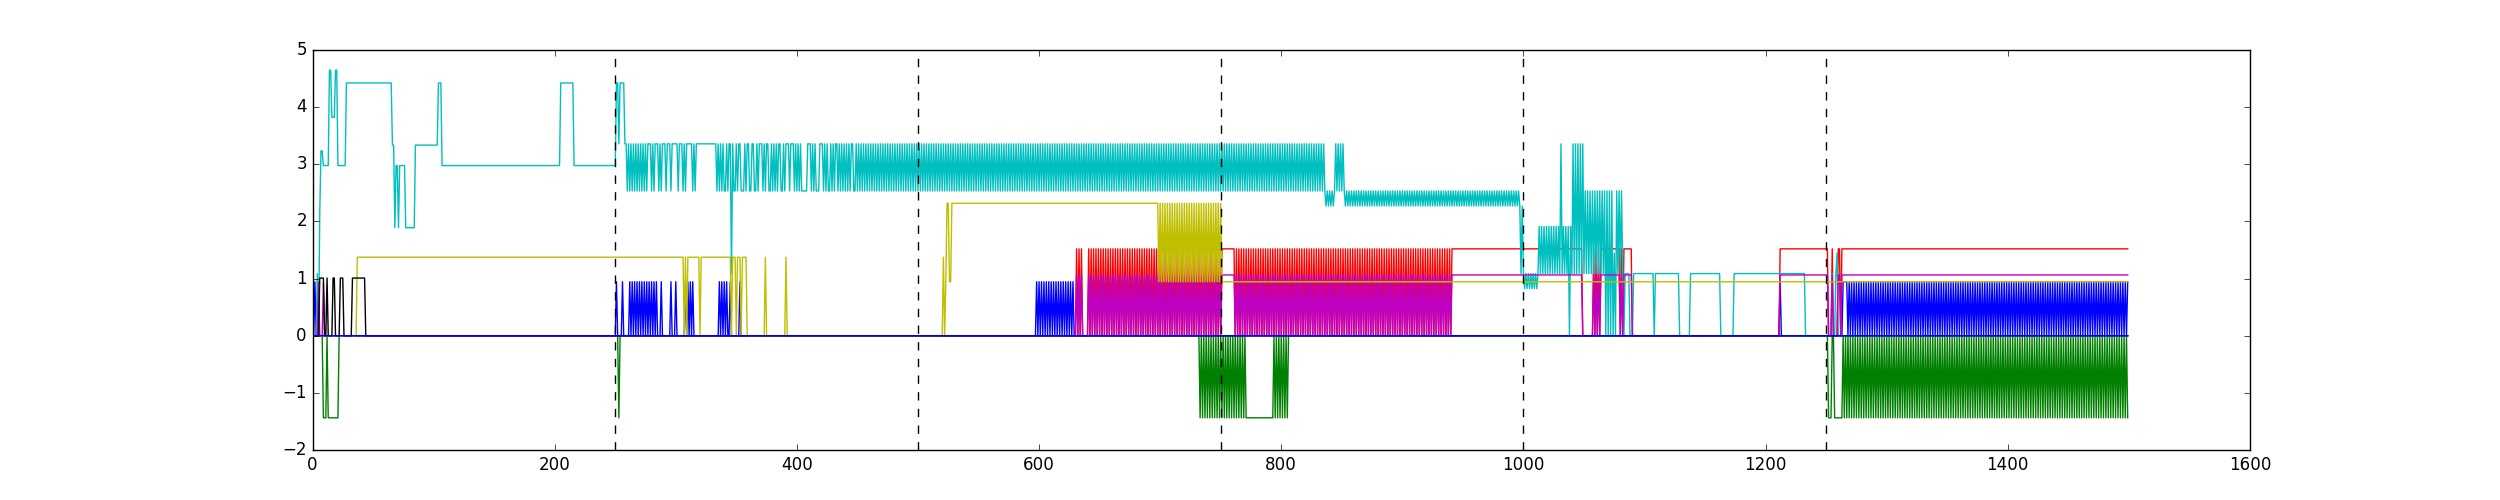
\includegraphics[width=\linewidth]{../visualizations/8knodes_unrandomized.png}
    \caption{Sensor and Output Graph (not primed)}
    \label{fig:unprimed_sensoroutput_graph}
\end{figure}

In this graph of output values as a function of sensor statuses, we set up a network with two sensors and six outputs, with all neurons in the net set to zero.  Initially, we turned on both sensors (causing all neurons connected to the sensors to fire), and ran this for 250 frames.  We then proceeded to switch the two sensors on and off, causing fluctuations in the output values.  As shown, turning off sensors affected the outputs as well as turning on sensors, and output values would sometimes cycle between two values once a stable point had been reached.  We believe that the cycling is due to a node signal cycle similar to one described earlier, with only part of the cycle contributing to the output loop.  Additionally, we believe the sensor deactivation effect is due to certain inhibitory neurons being disabled after the sensor is turned off.

Between any two nonadjacent cycle spans with the same sensors on, we can see that the stable values for neurons is often different.  We may be able to describe this with a similar process in biological brains \cite{synapticlearning,synapticpruning}, where synaptogenesis and synaptic pruning, alongside Hebbian learning, occur to modify neuron paths. 

\begin{figure}[H]
    \centering
    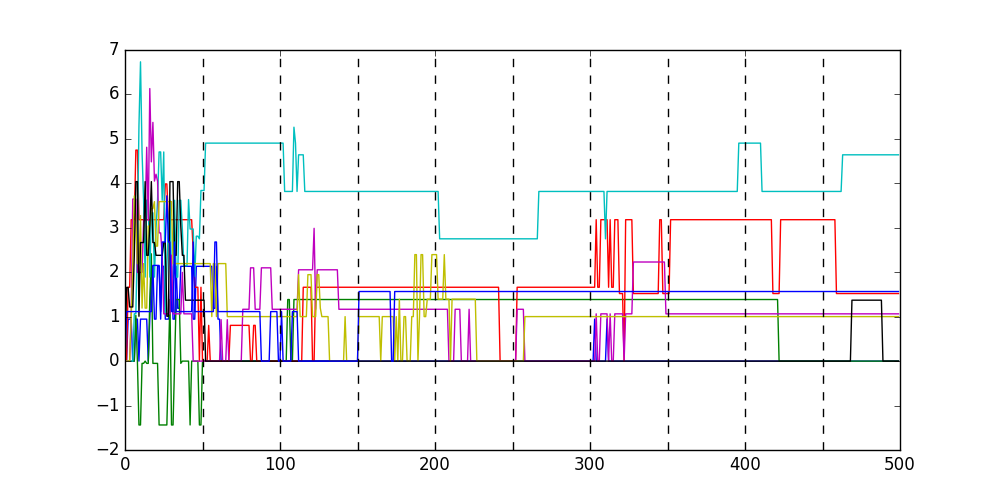
\includegraphics[width=\linewidth]{../visualizations/8knodes_quick_changes.png}
    \caption{Sensor and Output Graph (quick changes)}
    % \label{fig:unprimed_sensoroutput_quick_graph}
\end{figure}

In another exploration, we created another network with the same number of sensors and outputs, but we randomized all of the nodes before running any cycles.  In this case, we toggled sensor statuses every 50 cycles.  As illustrated, after the initial fifty cycles, the output values stabilized until a sensor was toggled on or off.  This result mirrors the result in Figure 5.  However, having less time to stabilize between two primary values in any given fifty-cycle chunk resuled in what seems to be more variation.  More rigorous analysis should be done over more generated networks to determine how significant this is.

\begin{figure}[H]
    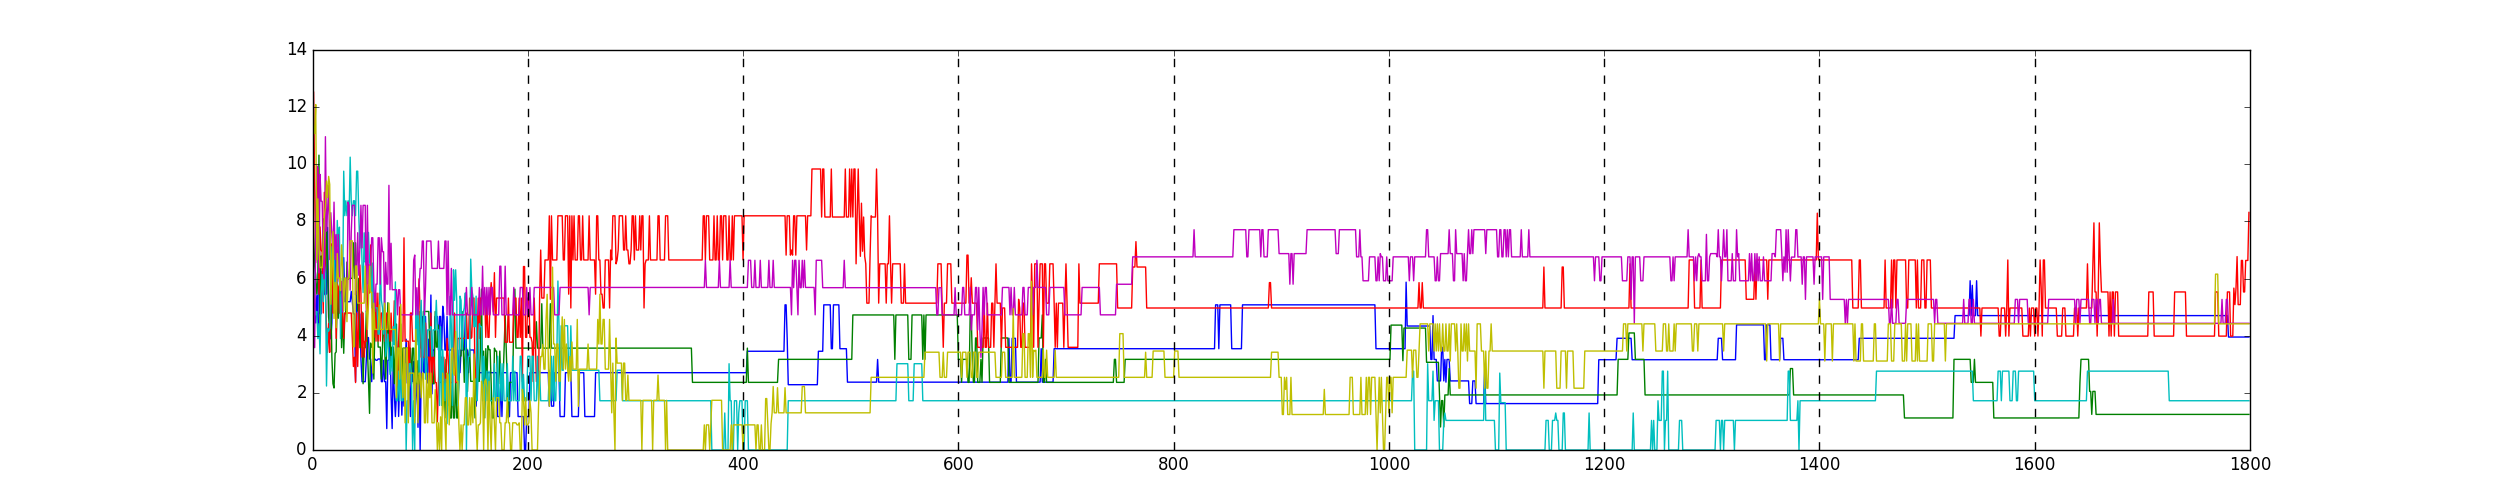
\includegraphics[width=\linewidth]{../visualizations/8knodes_sensors_lineannotated.png}
    \caption{Randomized (with inputs)}
    % \label{fig:unprimed_sensoroutput_graph}
\end{figure}

Another run, we randomized the network, with each space between the dotted lines indicating a set of input values was held constant (only changing at the dotted lines).  We can see that in the first 200 cycles, the output values lessened, until the inputs were initially activated.  This network, being different from the previous network, had less chaotic patterns in the graph.  However, we suspect that the major changes (deviating from the standard cycling) past cycle 200 are primarily due to the propagation of input data, as seen more clearly in Figures 5 and 6.  Once the input data were modified, it appeared as if the average output value also changed as long as the input data then remained constant, regardless of whether inputs were turned on or off.  Note that this change in output values occurred for both inputs that were turned on and inputs that were turned off.

Given these graphs, we may see, purely visually, that sensors do not affect their outputs immediately; there is always a nonzero time between sensor toggling and outputs being changed.  We propose that is it possible to use Granger causality analysis to analyze this behavior, as it has been shown to be successful, in some cases, in neuroscience \cite{neurocausality, netcausality}.  It would then be possible to establish a link between input values and output behavior, especially useful in cases of a primed network where it may not be easy to visually determine when or how sensors affect outputs.

Interestingly, these graphs somewhat resemble "brain waves" (e.g. EEG graphs), or neural oscillations, which have been observed in human brains and have been implicated in memory \cite{oscillationmemory} as well as low-level functions such as a "gating function" \cite{oscillations}.  In section \ref{looping}, we have discovered a similar process as occurs the described "gating function", which may be extended to act as an actual "gating function" due to signals from inhibitory neurons.  For example, consider the following figure where - denotes an inhibitory connection and + denotes an excitatory connection.

\begin{figure}[H]
    \centering
    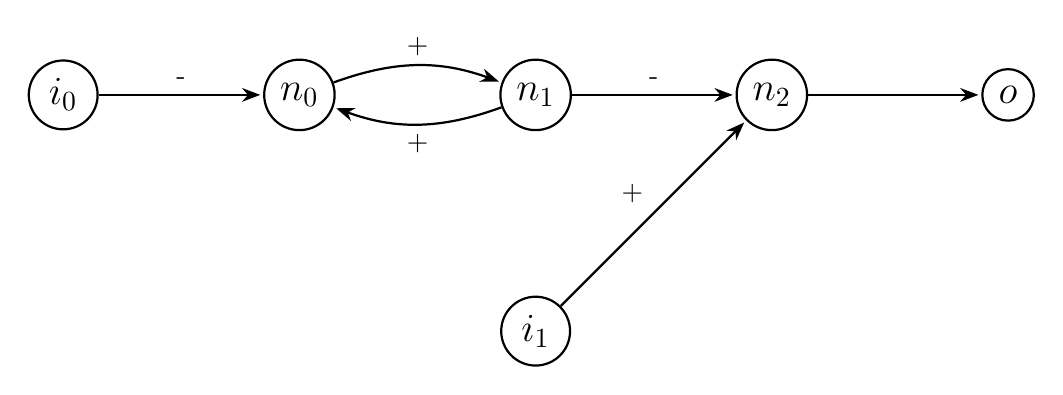
\begin{tikzpicture}[->,>=stealth',shorten >=1pt,auto,node distance=3cm,
                        thick,main node/.style={circle,draw,font=\sffamily\Large\bfseries}]

        \node[main node] (n1) {$n_1$};
        \node[main node] (n0) [left of=n1] {$n_0$};
        \node[main node] (n2) [right of=n1] {$n_2$};
        \node[main node] (i0) [left of=n0] {$i_0$};
        \node[main node] (i1) [below of=n1] {$i_1$};
        \node[main node] (o) [right of=n2] {$o$};

        \begin{scope}[>={Stealth[black]}]
            \path [->] (i0) edge node {-} (n0);
            \path [->] (n0) edge[bend left=20] node {+} (n1);
            \path [->] (n1) edge[bend left=20] node {+} (n0);
            \path [->] (n1) edge node {-} (n2);
            \path [->] (i1) edge node {+} (n2);
            \path [->] (n2) edge node {} (o);
        \end{scope}
    \end{tikzpicture}
    \caption{Gating} \label{fig:Gating}
\end{figure}

If a loop already exists between $n_0$ and $n_1$, and $i_1$ excites $n_2$, it is entirely possible that the value of the output $o$ remains zero.  However, if $i_0$ inhibits $n_0$ while $i_1$ excites $n_2$, it is also possible that the value of the output $o$ is nonzero.  This would be caused by the inhibition of $n_0$ breaking the loop with $n_1$, causing $n_2$ to lose its inhibitory influence and allowing it to fire when excited.


\subsection{Future Work} \label{future}

At the moment, our simulation runs in $\mathbb{R}^3$ space.  However, it is entirely possible that we may run it in $\mathbb{R}^n$ space for any $n \in \mathbb{N}$, given our method of node positioning and connection generation.  However, we postulate that this system is ineffective for $n=1$ and potentially $n=2$, as a higher $n$ allows for a higher level of complexity (e.g. more complex pattern combinations).  However, this causes a network to grow in complexity exponentially, so ideally we would have some faster or optimized method of computing cycles.

A known flaw of the model is that organic neurons may have varied firing rates \cite{firingrates}, while our simulation has constant firing rates.  However, this is merely an engineering problem that has not been implemented due to potential efficiency issues.  Future iterations should ideally implement varied neuron firing rates.

Furthermore, one drawback of the current model is that it has a heavy reliance on magic numbers, as illustrated by the large number of arbitrary constants throughout this paper.  Further research into how synapses grow, change, and die throughout an organism's lifetime is necessary to refine these constants, along with the more general concept of how axons grow and "seek" targets (likely more complex than a simple probability sphere).  Additionally, our priming method (section \ref{priming}) is primarily designed to explore the effect of chaotic preexisting patterns on input/output patterns, as opposed to modeling the initial brain state; however, we also have proposed, in the same section, the possibility that we may not require priming at all.  Again, further research must be done to determine how to effectively initialize the signals in the network.  Another drawback is that we do not take into account synaptic fatigue \cite{synapticfatigue}, which may be easily implemented in a rudimentary way by setting a neuron's "neurotransmitter count" and decreasing it by some number $n_l$ every time it fires, and then increasing it by some number $n_i < n_l$ every cycle.


\newpage

\section{Graphs and Data} \label{graphs}

\begin{figure}[H]
    \centering
    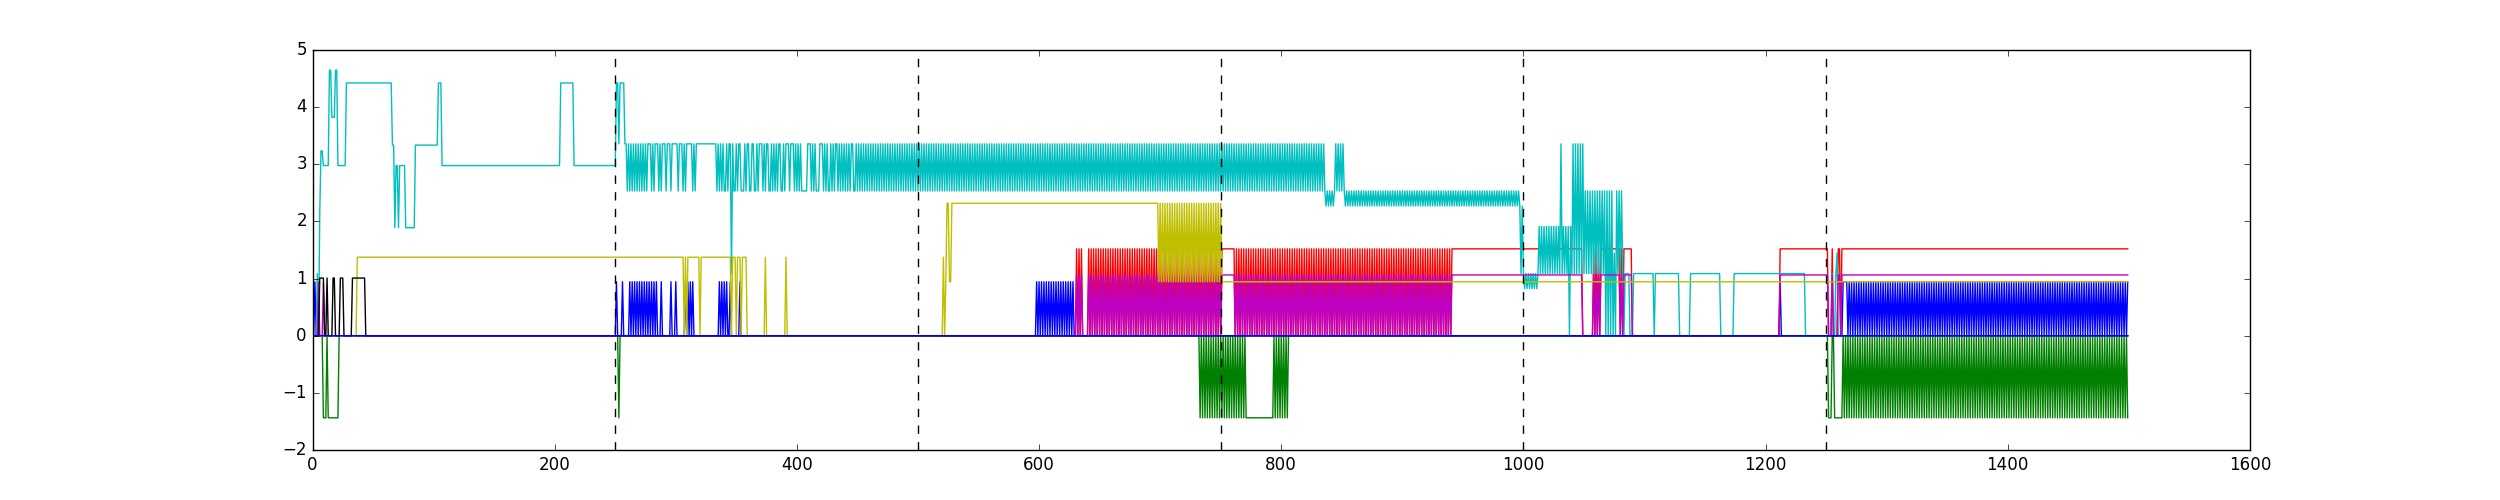
\includegraphics[width=\textheight,angle=270,keepaspectratio]{../visualizations/8knodes_unrandomized.png}
    \caption{Sensor and Output Graph (not primed)}
    % \label{fig:unprimed_sensoroutput_graph}
\end{figure}

\begin{figure}[H]
    \centering
    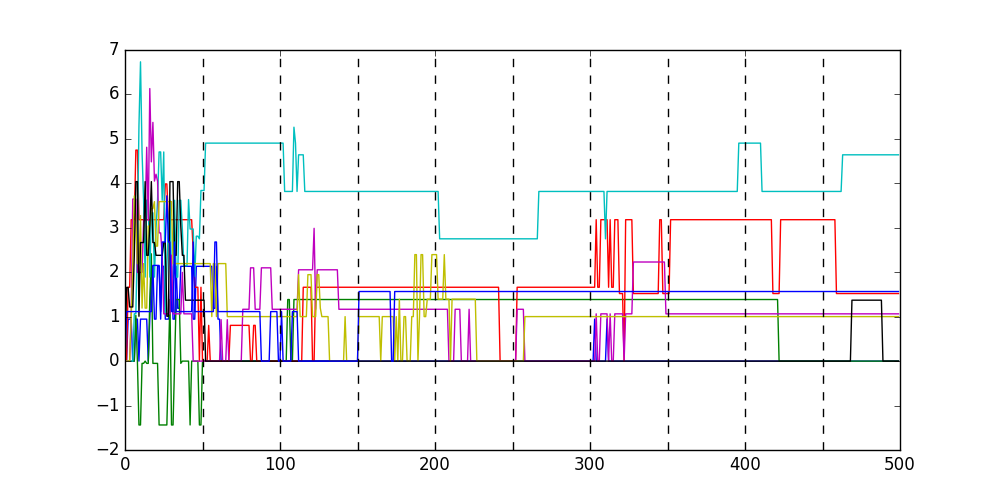
\includegraphics[width=\textheight,angle=270,keepaspectratio]{../visualizations/8knodes_quick_changes.png}
    \caption{Sensor and Output Graph (quick changes)}
    % \label{fig:unprimed_sensoroutput_quick_graph}
\end{figure}

\begin{figure}[H]
    \centering
    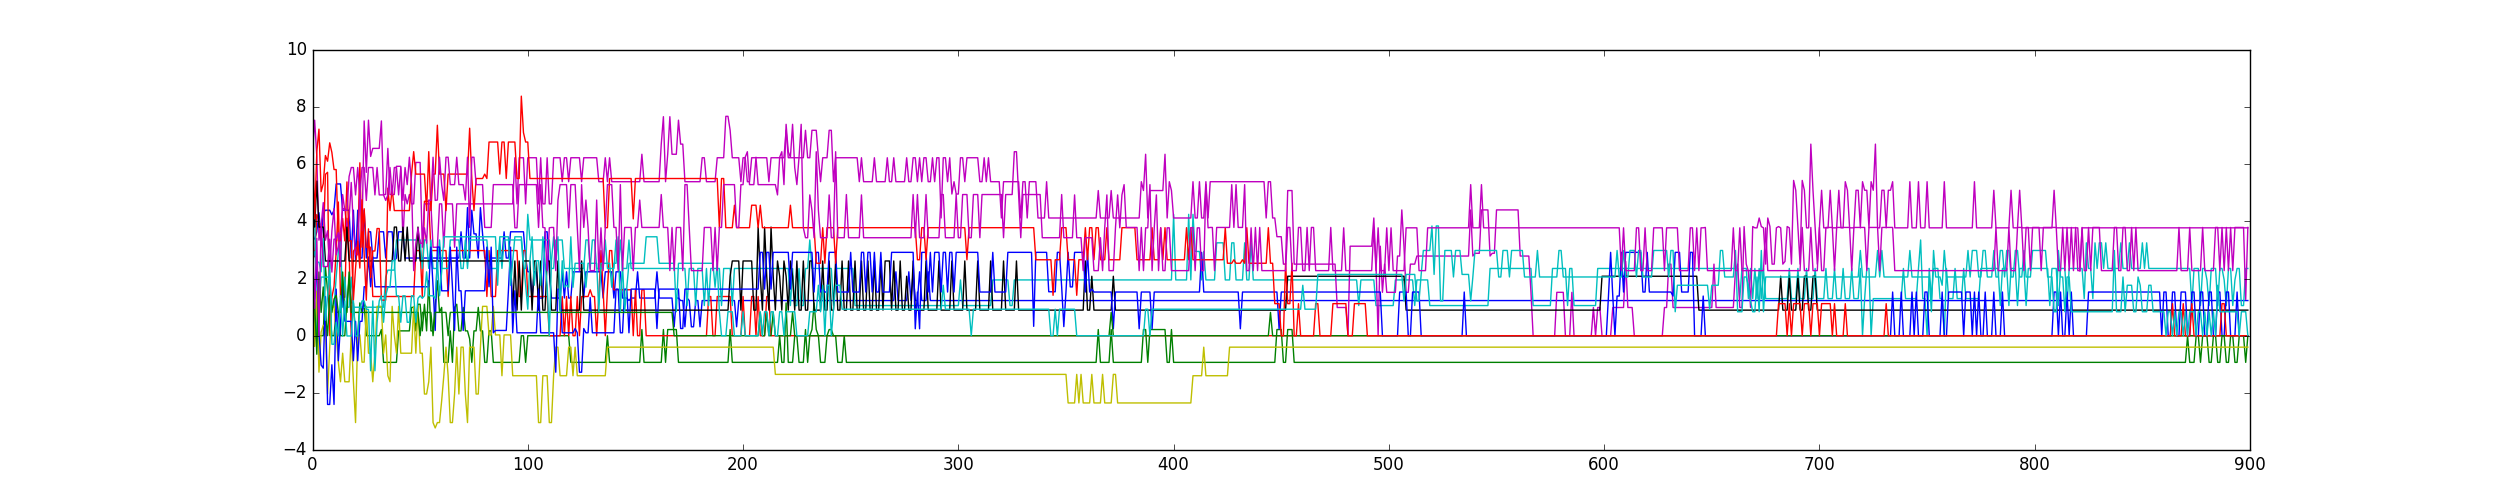
\includegraphics[width=\textheight,angle=270,keepaspectratio]{../visualizations/8knodes_stable_line.png}
    \caption{Randomized (no inputs)}
    % \label{fig:unprimed_sensoroutput_graph}
\end{figure}

\begin{figure}[H]
    \centering
    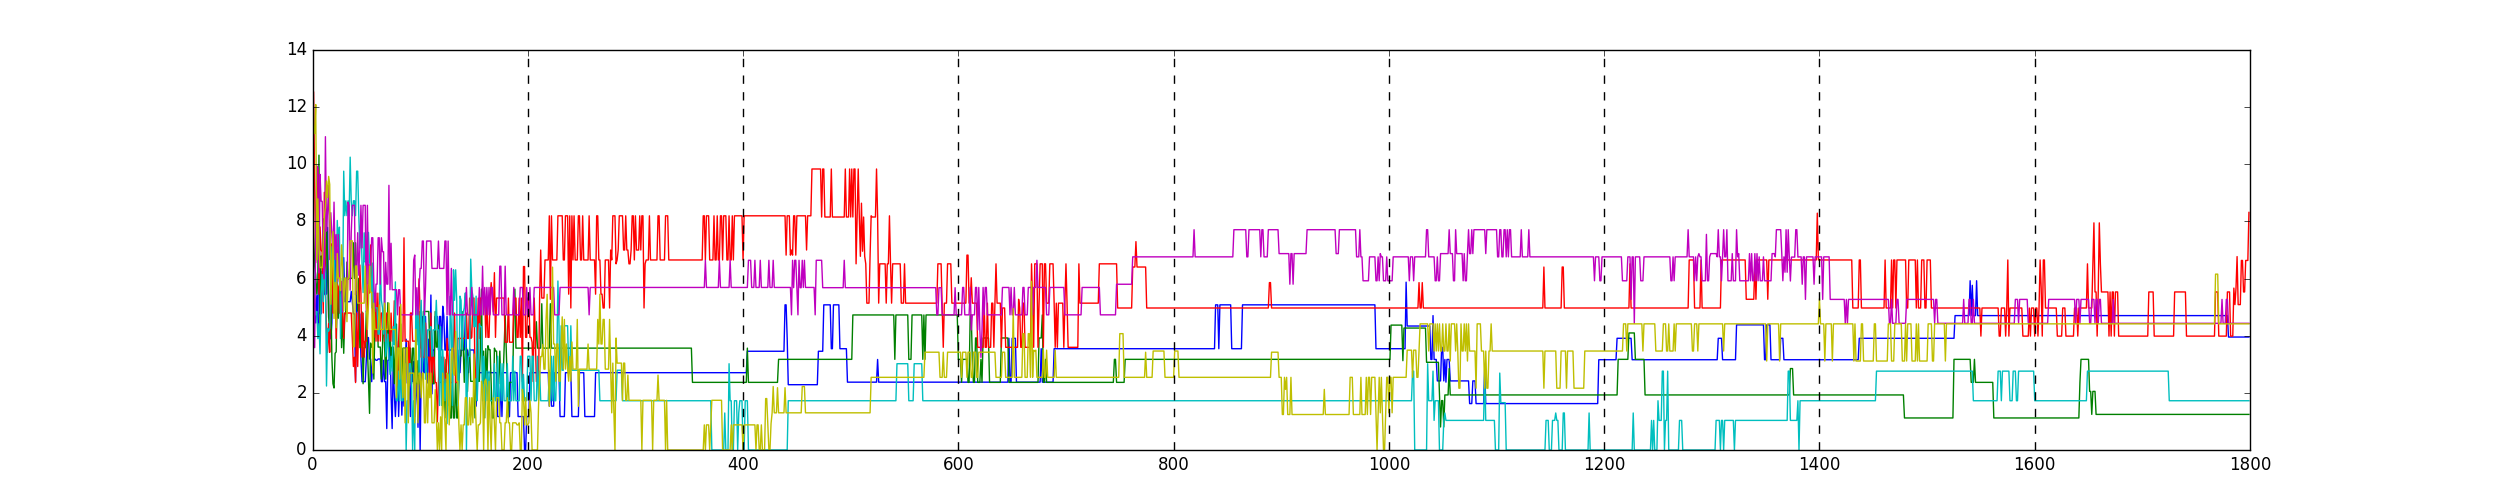
\includegraphics[width=\textheight,angle=270,keepaspectratio]{../visualizations/8knodes_sensors_lineannotated.png}
    \caption{Randomized (with inputs)}
    % \label{fig:unprimed_sensoroutput_graph}
\end{figure}


\newpage

\section{References}

% \nocite{*}
\printbibliography[heading=none]

\end{document}